\documentclass[conference]{IEEEtran}
\IEEEoverridecommandlockouts
% The preceding line is only needed to identify funding in the first footnote. If that is unneeded, please comment it out.
\usepackage{cite}
\usepackage{amsmath,amssymb,amsfonts}
\usepackage{algorithmic}
\usepackage{graphicx}
\usepackage{textcomp}
\usepackage{xcolor}
\def\BibTeX{{\rm B\kern-.05em{\sc i\kern-.025em b}\kern-.08em
    T\kern-.1667em\lower.7ex\hbox{E}\kern-.125emX}}
\setlength{\parindent}{0pt}
\begin{document}

\title{Network Security Lab 3: Packet Tracer – Configuring IPv6 Addressing}

\author{\IEEEauthorblockN{Alexander Hoffmann}
\IEEEauthorblockA{\textit{ECE Paris}\\
Paris, France \\
alexander.hoffmann@edu.ece.fr}
}

\maketitle

\section{Configure IPv6 Addressing on the Router}

\subsection{Enable the router to forward IPv6 packets}

\textbf{a.} Enter the ipv6 unicast-routing global configuration command. This command must be configured to enable the router to forward IPv6 packets.
\begin{verbatim}
# ipv6 unicast-routing
\end{verbatim}

\subsection{Configure IPv6 addressing on GigabitEthernet0/0}

\textbf{d.} We configure the IPv6 of R1 address with the following command:
\begin{verbatim}
# ipv6 address 2001:DB8:1:1::1/64
\end{verbatim}

\textbf{e.} We configure the link-local IPv6 address with the following command.
\begin{verbatim}
# ipv6 address FE80::1link-local
\end{verbatim}

\subsection{Configure IPv6 addressing on GigabitEthernet0/1}
Do the same as before except the change the IP address. For this router, the interfaces are described in Fig. \ref{router}.
\begin{verbatim}
# ipv6 address 2001:DB8:1:2::1/64
\end{verbatim}

\subsection{Configure IPv6 addressing on Serial0/0/0}
Here, we configure the serial interface of the router.

\begin{center}
\begin{figure}[h]
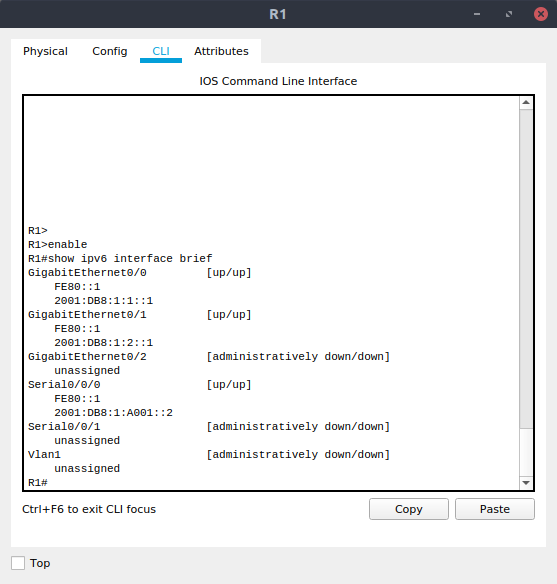
\includegraphics[scale=0.45]{resources/q1.png}\
\caption{IPV6 configuration for R1 interfaces}
\label{router}
\end{figure}
\end{center}

\section{Configure IPv6 Addressing on the Servers}
Set the IPv6 Address to 2001:DB8:1:1::4 with a prefix of /64. Set the IPv6 Gatewayto the link-local address, FE80::1. The configuration is shown in Fig. \ref{server_acc}.

\begin{center}
\begin{figure}[h]
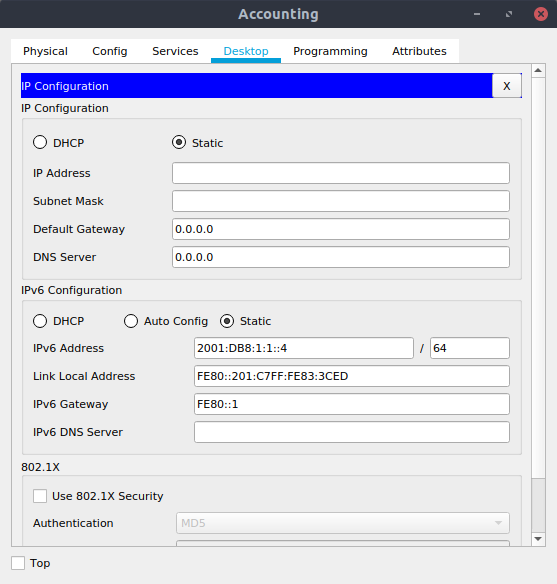
\includegraphics[scale=0.45]{resources/q21.png}\
\caption{Configuration of the accounting server}
\label{server_acc}
\end{figure}
\end{center}

We do the same for the CAD server which is printed in Fig. \ref{server_cad}.

\begin{center}
\begin{figure}[h]
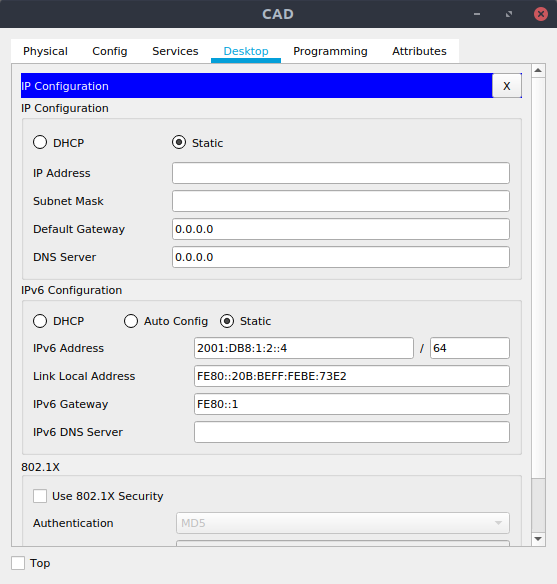
\includegraphics[scale=0.45]{resources/q22.png}\
\caption{Configuration of the CAD server}
\label{server_cad}
\end{figure}
\end{center}

\section{Configure IPv6 Addressingon the Clients}

\subsection{Configure IPv6 addressing on the Sales and Billing Clients}
Set the IPv6 Address to 2001:DB8:1:1::3 with a prefix of /64 and set the IPv6 Gateway to the link-local address, FE80::1. This is shown in Fig. \ref{client_billing}. Same for the sales client in Fig. \ref{client_sales}.

\begin{center}
\begin{figure}[h]
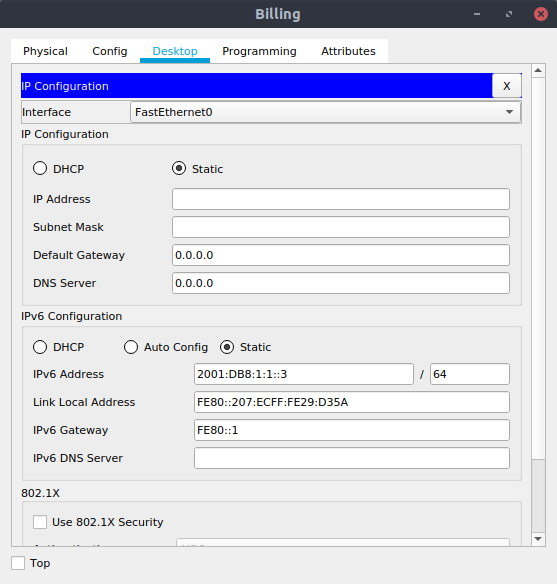
\includegraphics[scale=0.45]{resources/q31.png}\
\caption{Configuration of the billing client}
\label{client_billing}
\end{figure}
\end{center}

\begin{center}
\begin{figure}[h]
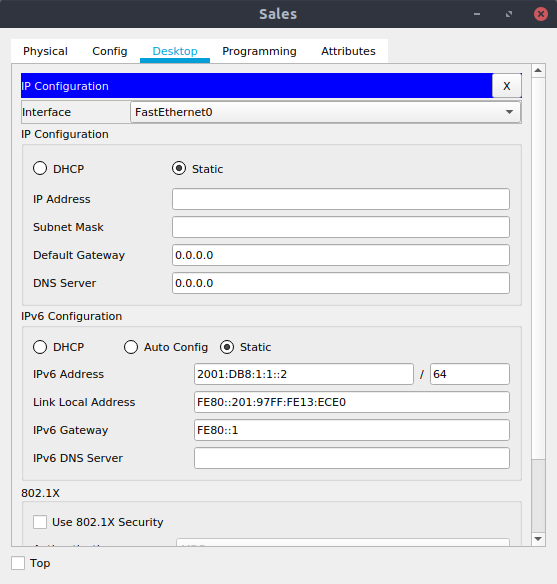
\includegraphics[scale=0.45]{resources/q32.png}\
\caption{Configuration of the sales client}
\label{client_sales}
\end{figure}
\end{center}

\subsection{Configure IPv6 Addressing on theEngineering and Design Clients}
Set the IPv6 Address to 2001:DB8:1:2::3 with a prefix of /64 and the IPv6 Gateway to the link-local address, FE80::1. Result is on Fig. \ref{client_engineering}. Same for the design client shown in Fig. 

\begin{center}
\begin{figure}[h]
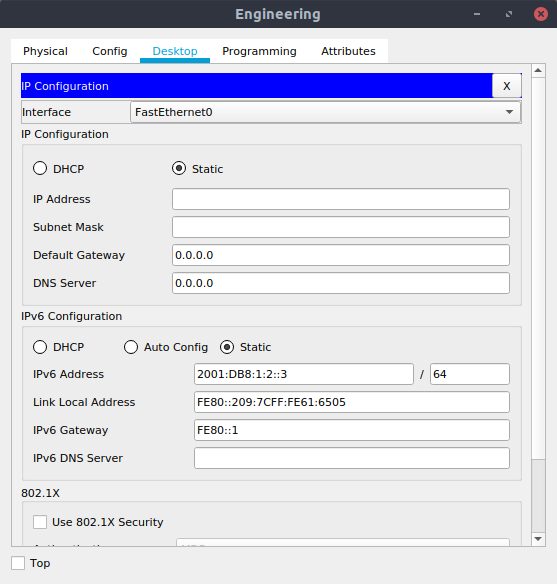
\includegraphics[scale=0.45]{resources/q33.png}\
\caption{Configuration of the engineering client}
\label{client_engineering}
\end{figure}
\end{center}

\begin{center}
\begin{figure}[h]
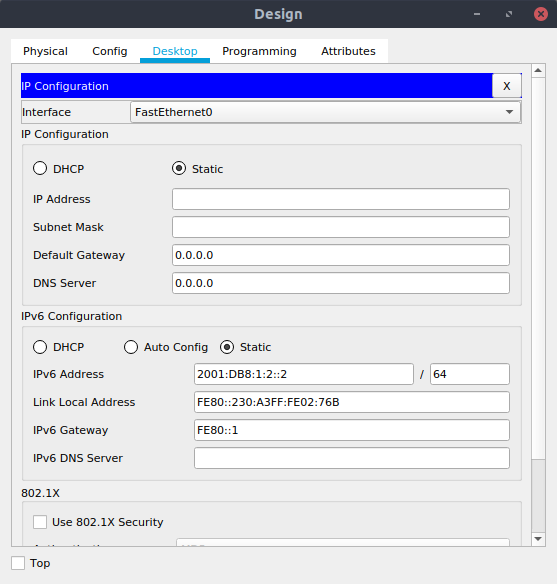
\includegraphics[scale=0.45]{resources/q34.png}\
\caption{Configuration of the design client}
\label{client_design}
\end{figure}
\end{center}

\section{Test and Verify Network Connectivity}

\subsection{Open the server web pages from the clients}
Go to accounting and CAD websites from sales desktop in Fig. \ref{browser_sales1} and Fig \ref{browser_sales2}.

\begin{center}
\begin{figure}[h]
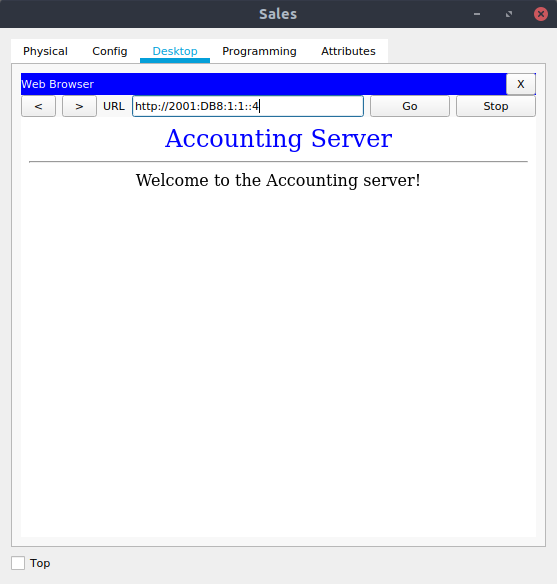
\includegraphics[scale=0.45]{resources/q41.png}\
\caption{Go to Accounting website}
\label{browser_sales1}
\end{figure}
\end{center}

\begin{center}
\begin{figure}[h]
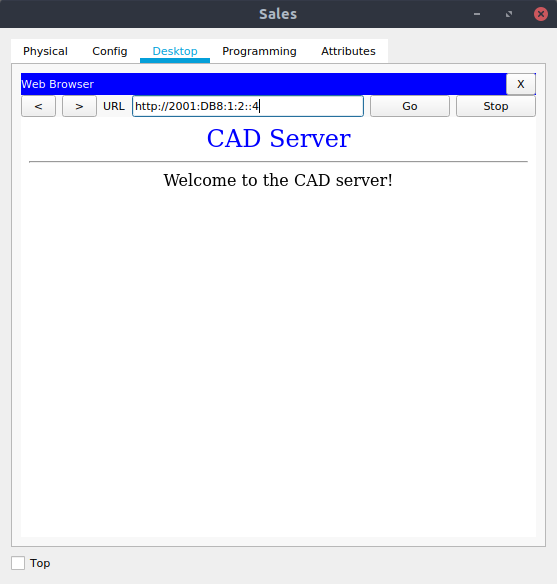
\includegraphics[scale=0.45]{resources/q42.png}\
\caption{Go to CAD website.}
\label{browser_sales2}
\end{figure}
\end{center}

Same for the design desktop in Fig. \ref{browser_design1} and \ref{browser_design2}.

\begin{center}
\begin{figure}[h]
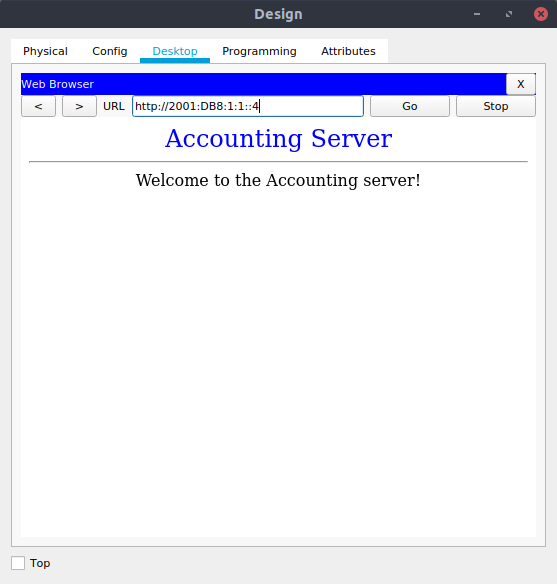
\includegraphics[scale=0.45]{resources/q43.png}\
\caption{Go to Accounting website}
\label{browser_design1}
\end{figure}
\end{center}

\begin{center}
\begin{figure}[h]
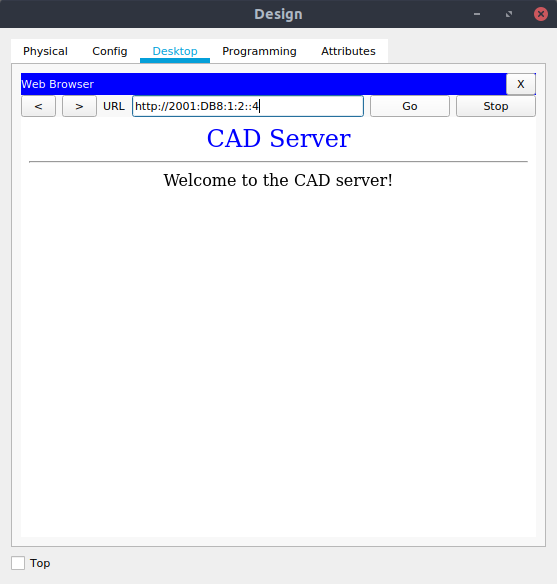
\includegraphics[scale=0.45]{resources/q44.png}\
\caption{Go to CAD website.}
\label{browser_design2}
\end{figure}
\end{center}

\subsection{Ping the ISP}
\begin{center}
\begin{figure}[h]
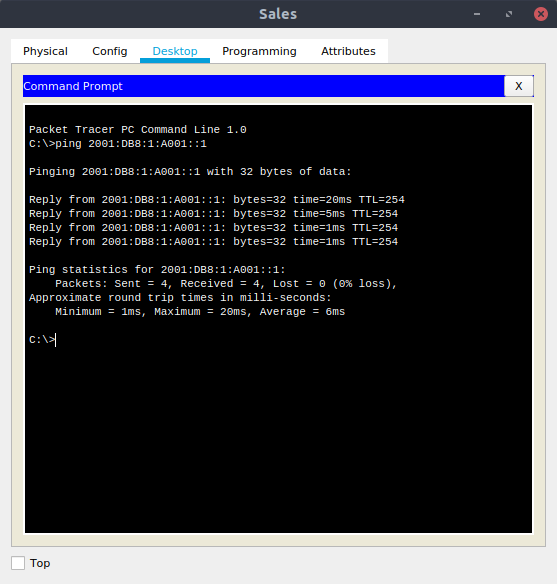
\includegraphics[scale=0.45]{resources/q422.png}\
\caption{Ping the ISP from Sales laptop.}
\end{figure}
\end{center}

\begin{center}
\begin{figure}[h]
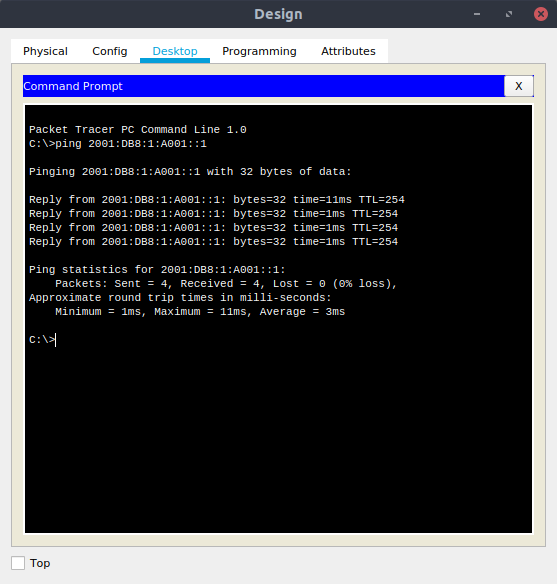
\includegraphics[scale=0.45]{resources/q423.png}\
\caption{Ping the ISP from Design	 laptop.}
\end{figure}
\end{center}

\end{document}
